\subsection*{Historical measurement and reproduction}

The original script classifies browsers by scanning punctuation-stripped strings for broad substrings, including \texttt{98}, \texttt{iphone}, and \texttt{firefox30}. That rule can match unrelated digits, mistake a secondary Internet Explorer token for the primary one, and miss older Firefox versions. The revised historical parser reads explicit version tokens and preserves unknowns. The full specification comparison is shown in Figure~\ref{fig:historical}; all definitions are exploratory sensitivities using overlapping records.

\begin{figure}[htbp]
\centering
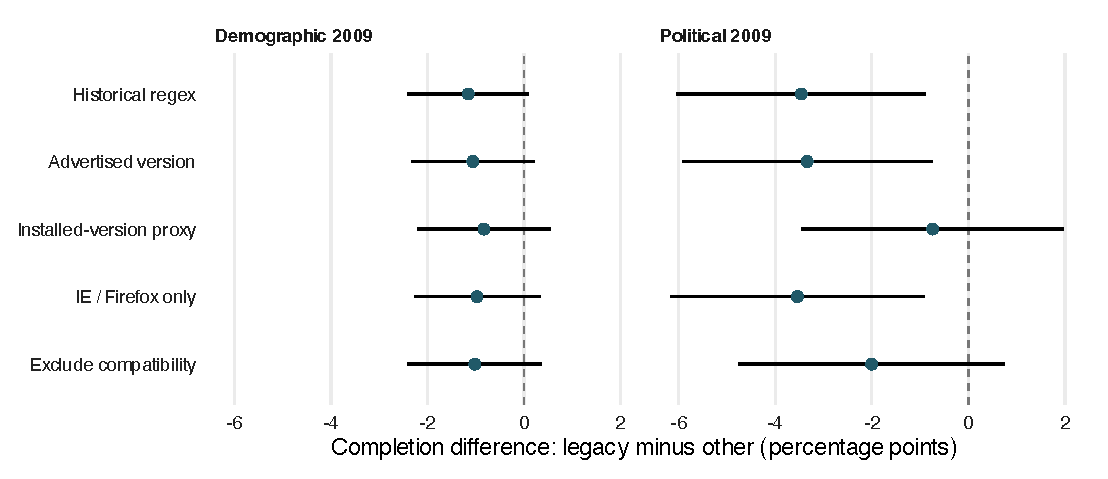
\includegraphics[width=\linewidth]{../figs/completion.pdf}
\caption{Historical completion differences under alternative browser definitions. Points compare legacy and comparator completion; lines show 95\% HC2 normal intervals. Each survey component uses its own observed starters. Unknown strings are excluded except under the historical regex. The panels are dependent samples.}
\label{fig:historical}
\end{figure}

The original SPSS exports confirm the source identities and every linked status and trimmed user-agent value. They establish that the demographic component is \texttt{.x} and the political component is \texttt{.y}; the earlier note reversed those labels. The older README's December--January invitation account does not match the October field timestamps. Invitation totals and population representativeness cannot be established from this extract. These provenance corrections do not supply missing pre-survey demographic information.

The original missing-data outcome counts \texttt{NA} cells across all \MergedColumns{} merged-file columns, mixing routing, absent components, metadata, experimental branches, and derived fields. It excludes empty strings. The revised fixed-field outcome is therefore a different quantity, not simply a corrected estimate of the same construct. Table~\ref{tab:blanks} reports the limited fixed-field sensitivity among completers.

\begin{table}[htbp]
\centering
\caption{Fixed-field blanks among historical survey completers.}
\label{tab:blanks}
\small
\begin{tabular}{lrrrrrr}
\toprule
Survey & Year & Fields & $N$ & Legacy & Other & Difference [95\% CI] \\
\midrule
Demographic & 2009 & 9 & 2009 & 0.003 & 0.002 & 0.002 [-0.004, 0.007] \\
Political & 2009 & 5 & 2055 & 0.005 & 0.011 & -0.006 [-0.015, 0.003] \\
\bottomrule
\end{tabular}

\par\smallskip
\begin{minipage}{\linewidth}\footnotesize
\emph{Note}: Means count blank fields per person, including whitespace-only text. Explicit don't-knows count as recorded answers. Demographic fields cover handedness, state, gender, household composition, birth month/year, marital status, education, and Hispanic origin; political fields are the knowledge questions. Intervals use HC2 standard errors. Unknown browser versions are excluded. Question-level exposure is unverified, so these are not all-question item-nonresponse rates.
\end{minipage}
\end{table}

The 2023 adjusted missing-cell models retain the same \HistoricalMissingN{} people and return the same browser coefficient, \HistoricalMissingGap{} ($p=\DemMissingP{}$). The 2011 models instead use different samples and duration restrictions. Their completion tests reproduce $p=\DemNoteP{}$ and $p=\PolNoteP{}$; the 2023 completion tests give $p=\DemOldP{}$ and $p=\PolOldP{}$. These are specification changes rather than a failure to reproduce the earlier arithmetic.

\subsection*{Checks and reproducibility}

For a two-group mean difference, HC2 variance equals the sum of the two sample variances divided by their group sizes \citep{sandwich}. Independent arithmetic checks, alternative logistic summaries, Fisher tests, deletion influence, and all allocations of unknown browser statuses are in the replication outputs. Seeded simulations assess interval behavior under independent Bernoulli sampling, not the sample's representativeness. Sparse July differences use Newcombe intervals derived from Wilson limits, checked independently from their group counts. The duration quartiles are descriptive distribution summaries rather than uncertainty intervals. For March narrative responses, we average the two common questions within each person before computing Welch intervals from group means and variances. Browser-family intervals are exploratory and unadjusted for multiple comparisons; word counts, log-transformed person means, question-specific summaries, and single-record deletion bounds are retained in the replication outputs.

The expanded analysis keeps source-specific imports separate from the shared technical and outcome definitions. The item/timer map, source hashes, duplicate checks, measurement ledger, and retrospective analysis plan are recorded in the repository. Source imports write aggregate summaries only. The ordinary build regenerates question-organized tables, figures, and manuscript numbers from the historical data and those aggregates; rebuilding the aggregate snapshots requires the authorized sibling exports and downloaded public corpus.
